\section{Methods}\label{section:Methods}

\subsection{Mesh generation}\label{section:Mesh}
To discretize the 2D subsurface geometry, especially the diatreme structure, as good as possible an unstructured, triangular mesh is used. This is done in PyGIMLI by using the function \textit{pygimli.meshtools.createMesh()} which is calling the two-dimensional quality mesh generator and Delaunay triangulator \textit{Triangle} \citep{shewchuk1996triangle}. The resulting mesh is shown inf Figure \ref{figure:mesh} and consists mainly of triangles without small and large angles and is therefore suitable for finite element calculations. The big benefit of the unstructured mesh is that it can discretize curved or irregular boundaries better than a rectangular grid and therefore ensures a better accuracy when running calculations on the model. A discretization of the diatreme structure with a rectangular grid would result in steps at the boundaries, rectangular grids were not considered.

Different material properties, i.e. seismic P-wave velocity, electrical resistivity and density, are assigned to the  different geologic formations that are indicated in Figure \ref{figure:synthetic_model}. The values are based on previous geophysical studies of the area as for example \citet{NiklasPlumpe.2015,TimGilberti.2020} and further literature like \citet{geldart2004problems,palacky1988resistivity} and summarized in table \ref{table:properties}. The upper sandstone layer (SS) is assumed to be part of the groundwater aquifer and therefore has a much lower resistivity than the more consolidated and dense sandstone layer below (CSS). This model will be used as an input for the gravimetric, ERT and traveltime tomography forward calculations which are presented in the following sections.

\begin{table}[]
\caption{Material properties of different geologic formations.}
\centering
\begin{tabular}{lccc}
%{m{15mm} m{70mm} m{18mm}}
\hline 
\textbf{Formation} & \textbf{P-wave Velocity}  & \textbf{Electrical Resistivit}  & \textbf{Density}  \\
& \textbf{[$m/s$]}  & \textbf{[$\Omega m$]}  & \textbf{[$kg/m^3$]}\\ \hline 
Soil & $650$ & $120$ & $1250$\\
SS & $3000$ & $1200$ & $2400$\\
CSS & $3600$ & $3500$ & $2500$\\
Basement & $4500$ & $10^8$ & $2650$\\
Diatreme & $2000$ & $10^5$ & $2100$\\
 \hline 
\end{tabular}
\label{table:properties}
\end{table}


\begin{figure}[]
  \centering
  \begin{minipage}[b]{0.48\textwidth}
    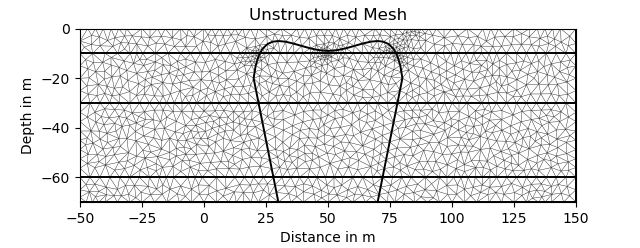
\includegraphics[width=\textwidth]{Figures/Mesh.png}
    \caption[Unstructured mesh]{Unstructured, triangular mesh used to discretize the subsurface geometry.}
    \label{figure:mesh}
  \end{minipage}
  \hfill
  \begin{minipage}[b]{0.48\textwidth}
    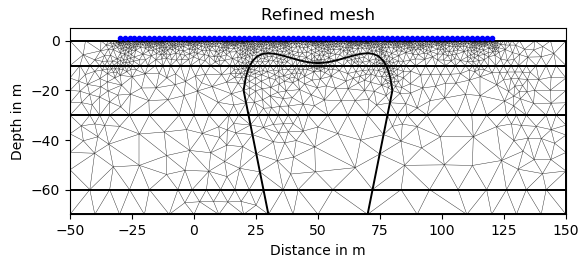
\includegraphics[width=\textwidth]{Figures/ERT_refined_mesh.png}
    \caption[Refined mesh used for ERT calculations]{Refined mesh used for ERT calculations. Here electrodes are between -20 and 120m.}
    \label{figure:refined_mesh}
  \end{minipage}
\end{figure}

\subsection{Electrical Resistivity Tomography}\label{section:ERT}
The ERT method is sensitive to electrical resistivity contrasts in the subsurface due to for example changes in clay content, porosity, pore fluid or ore minerals. First a direct current is inserted into the ground using two electrodes and then the potential difference between two points is measured with two additional electrodes. The electric potential $U$ can be calculated using the Poisson equation: 
\begin{equation}
    \nabla[\sigma (\textbf{r}) \nabla U(\textbf{r})] = -\nabla J
    \label{Eq:poisson}
\end{equation}

Here $\textbf{r}$ stands for the location, $J$ for the injected electrical current, and $\sigma$ for the electrical conductivity which is the inverse of the electrical resistivity $\rho$. This equation builds the basis for the ERT forward calculation \citep{johnson2015accurate}. For a known conductivity distribution, a known injected current and appropriate boundary conditions at the model boundaries, the potential at every location inside the model can be calculated. 

In PyGIMLI the calculation is performed using the module \textit{pygimli.physics.ert} which makes use of the open-source library BERT \citep{gunther20063, rucker20063}. It assumes a Neumann boundary condition (fixed derivation of the potential) for the upper boundary as its is representing the free surface boundary of the Earth. For the remaining boundaries a mixed boundary condition is implemented to avoid unpyhsical field distortions and ensure accuracy of the simulation. 
Using information defined in ert.scheme a finite element simulation can be run to determine the electrical potential in the modelling domain. To ensure numerical accuracy a refinement of the mesh is performed close to the current injection locations as well as the potential measurement locations. The refined mesh is shown in Figure \ref{figure:refined_mesh}. Note that the new mesh has smaller cells close to the surface where the virtual electrodes are located and bigger cells in greater depth. That is done to ensure higher accuracy close to injection points which is crucial for the whole simulation.

Using the results of the simulations the potential differences between two virtual electrodes for two virtual injecting electrodes can be calculated. This can be converted to apparent resistivity $rho_{app}$ according to \citet{kearey2002introduction} as follows:
\begin{equation}
    \rho_{app} = \frac{2\pi}{\frac{1}{\overline{AM}}-\frac{1}{\overline{AN}}-\frac{1}{\overline{BM}}+\frac{1}{\overline{BN}}} \frac{\Delta U}{I} = K \frac{\Delta U}{I}
    \label{Eq:rho_app}
\end{equation}

$\Delta U$ represents the potential difference between the two measurement locations $M$ and $N$, $I$ stands for the strength of the injected electrical current between the locations $A$ and $B$. The distance between an injection point and a measurement point is represented for example by $\overline{AM}$. The factor related to the acquisition geometry is called $K$ and is also often referred to as geometrical factor. To create a more realistic data set, noise is added to the data inside the \textit{simulate()} function. The noise is random and is defined by an absolute value as well as a noise level. The noise level is given in percent and defines the relative noise magnitude on a data point. The absolute noise on the other hand defines a noise magnitude independent from the data point and is therefore defined in the unity of volt $V$. For each data point the bigger of those noise criteria is chosen to define the noise that is contaminating the data.

After generating the synthetic data as described above an inversion is performed in order to turn the apparent resistivity section into a true resistivity distribution. This is done in PyGIMLI via the function \textit{pygimli.frameworks.methodManager.invert()}. This function requires the generated synthetic data as input as well as parameters for the inversion mesh generation and the inversion. The function is starting the inversion process by constructing an inversion mesh based on the acquisition geometry and the additional parameters given as an input. The inverse problem is subject to a non-linear optimization problem as the misfit function $\chi$ needs to be minimized. The misfit criterion $\chi$ is calculated using the synthetic data and the predicted data. A value of approximately $\chi=1$ is desirable as it represents a model that explains the data within the uncertainties. Using a Gauss-Newton algorithm a error-weighted, smoothness-constraint least-squares solution to the inverse problem is determined which can be visualized as a true resistivity distribution. The smoothness constraint is mainly defined through the regularization parameter $\lambda$ which weights between the data fit $\chi$ and the model smoothness. The higher the $\lambda$ value the smoother is the resulting model, however, it results in a worse data fit \citep{Ruecker2017}.

\subsection{Traveltime Tomography}\label{section:TT}
Traveltime tomography, also often referred to as seismic refraction tomography, is a method that is based on seismic refraction in the subsurface. Refracted waves can be observed if a seismic velocity increase can be observed with increasing depth. In that case the wave is travelling faster inside the deeper refractor in comparison with the direct wave which is travelling along the surface such that at a certain distance the refracted wave is overtaking the direct wave. Then the first arrival in the seismic measurements is contributed by the refracted wave \citep{kearey2002introduction}. Synthetic traveltime tomography data is created using the standard routine in the module \textit{pygimli.physics.traveltime}, starting with the setup of the acquisition geometry. Then, a refined mesh is constructed similar to the ERT calculations described in section \ref{section:ERT}. The synthetic data is then generated via the function \textit{pygimli.physics.traveltime.TravelTimeManager.simulate()} which computes the ray paths between sources and sensors. With known ray paths the synthetic data, i.e. the traveltimes, can be calculated according to \citet{zelt2021traveltime} as:
\begin{equation}
    t_i = \sum_j l_{ij}sj
    \label{Eq:TT}
\end{equation}

$t_i$ is the i-th taveltime observation, $l_{ij}$ the length of the i-th ray path segment (corresponding to the i-th observation) in the j-th model cell and $s_j$ is the slowness of the j-th model cell. Note that the slowness $s$ is the reciprocal of the velocity $v$. Noise can be defined similar as it was already described for the synthetic ERT data. Important to mention is that the absolute noise is defined in seconds ($s$) as traveltimes are generated.

After generating the synthetic traveltimes, an inversion of the data is performed similar to the ERT data inversion described in section \ref{section:ERT}. PyGIMLI performs an inversion of the traveltime data by calling the function \textit{pygimli.physics.traveltime.TravelTimeManager.invert()}. The result is, similar to the ERT inversion, an error-weighted, smoothness-constraint least-squares solution in form of a velocity model that explains the data within the uncertainties \citep{Ruecker2017}.


\subsection{Gravimetry}\label{section:Gravimetry}
The gravity method is based on Newton's Law of Gravitation which relates the force $F$ between two bodies with their masses $m_1$ and $m_2$ and the distance $r$ between them as:
\begin{equation}
    F = \frac{Gm_1 m_2}{r^2}
    \label{Eq:Newton1}
\end{equation}

The constant $G$ is called the gravitational constant and holds a value of $6.67*10^{-11}m^{3}kg^{-1}s^{-2}$. Assuming that one body is the Earth with a mass $M$ and a radius $R$, the gravitational force on an object on the Earth surface would be:
\begin{equation}
    F = \frac{GM}{R^2}m = gm
    \label{Eq:Newton2}
\end{equation}

As shown in the equation \ref{Eq:Newton2} the gravitational force on a body is a product of the gravitational acceleration $g$, often also referred to as gravity, and its mass. In gravimetry it is most useful to describe the gravitational field in form of its potential $U$ as the gravitational acceleration is the gradient of the potential $U$. The magnitude of the potential depends on the radius as well as on the density distribution in the subsurface and therefore measurements of the gravitational acceleration can be used to gain knowledge of subsurface structures \citep{kearey2002introduction}.

A synthetic gravity study of the simplified diatreme model is performed in PyGIMLI. This is achieved by applying the function \textit{pygimli.physics.gravimetry.solveGravimetry()} to the mesh with a defined sensor geometry and density distribution. The forward calculation of the gravimetric potential is the performed after \citet{won1987computing}. The synthetic data then shows then the gravitational response of the density distribution. To isolate the gravity response of the anomaly synthetic data of the layered subsurface without the diatreme structure will be generated and deducted from the first simulation data. The resulting data shows the effect of the diatreme structure on the gravitational acceleration, i.e. the first derivative of the gravitational potential. As PyGIMLI does not offer a fast and easy way yet to invert gravity data in 2D and due to the lack of time during the research module, the synthetic gravity data is not inverted in this work. However, the synthetic data will be visualized and discussed.

